\section{Preliminaries and Overview}
In this section we formalize the internals of a Deep CNN which will be later used to propose our incremental inference approach in Section 3. We then state the problem studied, explain our assumptions, and given an overview of \system.

\subsection{Deep CNN Internals}
CNNs are composed of a number of different layers: \textbf{convolution} layer, \textbf{pooling} layer (average or max pooling), \textbf{activation} layer, and \textbf{fully-connected} layer.

The main difference of CNNs compared to other neural networks is that they make the explicit assumption that the input is always going to be an image.
This assumption enables them to incorporate several architectural properties into the CNN architecture which reduce the amount of computations required for inference and the amount of learnable parameters.
Neurons in a particular layer of a CNN are organized into 3D volumes with width, hight, and depth dimensions.
For example the images in ImageNet dataset can be treated as an input volume of activations having dimensions of $224\times224\times3$.
Unlike in typical neural networks, a neuron in a convolution layer is only connected to a small region of the layer before it, instead of all the neurons in a full-connected manner.
However this is changed in the last layer (or last few layers) of a CNN in which a neuron is connected to all the neurons in the layer below in a fully connected manner. 

A Deep CNN is composed of several different types of layers. The main types used to build a CNN are: Convolutional Layer, ReLu Layer, Pooling Layer, Fully-Connected Layer and Softmax Layer. Usually Convolution and Fully-Connected are always followed by a ReLu layer which performs a activation wise function which outputs the max of zero of the weighted sum of activations of the connected neurons. Convolution and Pooling layers are stacked alternately to form a cascade of layers and at the end Full-Connected layers are used. A Softmax layer is used at the end of Fully-Connected Layers to output the class probabilities.
Generally in CNNs the activation volumes and filter maps, height and width of the spatial resolution is set to be the same producing square matrices.
Figure. \ref{fig:vgg16} demonstrates how these layers are stacked together to form VGG16 CNN architecture.
Next we will look into Convolutional and Pooling Layers in more detail.

\begin{figure}
  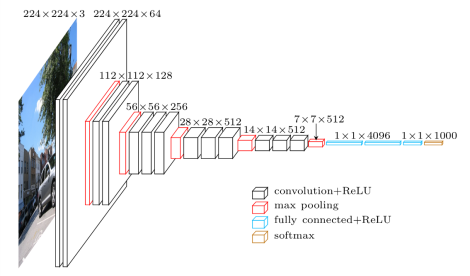
\includegraphics[width=\columnwidth]{./images/vgg16}
  \caption{VGG16 CNN Architecture}
  \label{fig:vgg16}
\end{figure}

\subsubsection{Convolutional Layer}
Convolutional Layer (Conv) is the most important type of layer in a CNN architecture. Also it is the most computationally intensive layer which accounts up to 90\% (or more) of the total computations in a Deep CNN model.
Conv layer parameters consist of set of learnable filters each of which has small spatial dimensions but extends across the depth of the input volume.
For example the first Conv layer of VGG16 model has 64 filter and each has a spatial dimension of $3\times3$ and a depth of $3$ (corresponding to the color depth of the image). In contrast the second Conv layer has 64 filters with the spatial dimension of $3\times3$ but with a depth of $64$ (the depth of the activation volume of layer 1).
A filter is convolved across the height and width dimensions of the input volume producing a 2D feature map where each activation is calculated by the dot product between the filter parameters and the activations of the input volume.
Note that here, only a small portion of the total activations in the input volume, which are spatially collocated together, are used to calculate the activation of an output neuron (see Figure. \ref{fig:conv_local_comp}).
Stacking the 2D feature maps produced for all the filter(e.g VGG16 first Conv layer has 64 filters) a output 3D activation map is created.
At the training time the parameters of the filters are updated using backpropagation and stochastic gradient descent such that these parameters learn to identify different visual concepts (eg. edges, color blotches, and high level objects such human faces) from the activation volume of the layer below \cite{zeiler2014visualizing}.

\begin{figure}
  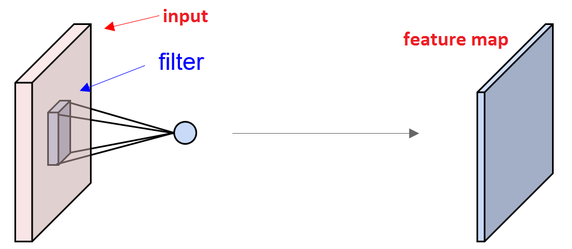
\includegraphics[width=\columnwidth]{./images/cnn_local_computation}
  \caption{Output feature map is computed by performing a dot product between filter values and the input activations}
  \label{fig:conv_local_comp}
\end{figure}

In addition to performing spatial convolutions, Conv layers can optionally reduce the spatial resolution of features volumes. Two hyper-parameters control the size of the output feature volume: the \textbf{stride}, and \textbf{zero-padding}.

\textbf{stride}: When moving the filter across the input volume a stride value has to be specified. When the stride is set to one, the filter is moved one pixel at a time. If the stride is larger than 1, for example setting it to two, the filter is moved 2 pixels at a time producing a smaller output spatial resolution.

\textbf{zero-padding}: Sometimes before performing the filter convolution it is beneficial to pad the input volume with zeros around the border to obtain the required output size. Also, by padding with zeros we can ensure that the input and output volumes will have the same spatial resolution when the stride is set to one.

Given the size of the input volume (\textbf{W}), size of the filter (\textbf{F}), amount of zero-padding (\textbf{P}), and the stride (\textbf{S}) the size of the output volume can be computed by (\textbf{W} - \textbf{F} + 2\textbf{P})/\textbf{S} + 1. For example in VGG16 first Conv layer, the input and output size is $\textbf{W}=224$ and the filter size is set to $\textbf{F}=3$ and is stride is set to $\textbf{S}=1$. To produce the output of same size the padding value should be set to $\textbf{P}=1$. Also note that the potential values for \textbf{W}, \textbf{F}, \textbf{P}, and \textbf{S} has mutual constraints as the output size has to be an integer.

\subsubsection{Pooling Layer}
CNNs architectures periodically insert Pooling Layers to mainly to reduce the spatial resolution of output features maps and also to introduce translational invariance to the image predictions. The pooling layer operated independently on each input feature map along the depth dimension and applies a local filter such as \textbf{max(...)}. The most typical form of Max Pooling is to apply a filter map of size $2\times2$ with a stride of 2 which reduces the height and width of the input feature map by a factor of 2 and discard $75\%$ of the activations. In general when applying a Pooling filter of size \textbf{F} on an input feature volume of size \textbf{W} with a stride of \textbf{S} the produced output volume will have a size of (\textbf{W} - \textbf{F})/\textbf{S} + 1.

\subsection{Computational Cost of Deep CNNs}
Deep CNNs are highly compute intensive and out of the different types of layers, Conv layers contributes to $90\%$ (or more) of the computations. One of the widely used way to estimate the computational cost of a Deep CNN is to estimate the number of fused multiply add (FMA) floating point operations (FLOPs) required for a single forward inference.

Conv layer producing an output feature map of size (\textbf{$W_2$}$\times$\textbf{$W_2$}$\times$\textbf{$D_2$}) from an input feature map of (\textbf{$W_1$}$\times$\textbf{$W_1$}$\times$\textbf{$D_1$}) using a filter of size (\textbf{$F$}$\times$\textbf{$F$}$\times$\textbf{$D_1$}) will require \textbf{$F$}$\times$\textbf{$F$}$\times$\textbf{$D_1$}$\times$\textbf{$W_2$}$\times$\textbf{$W_2$}$\times$\textbf{$D_2$} FMA operations.
For example in VGG16, computing a single activation of the first Conv volume requires 27 $(3\times3\times3)$ FMA operations and computing the whole output Conv volume requires 84 $(3\times3\times3\times224\times224\times64)$ Mega FMA operations. A Fully-Connected Layer reading \textbf{$N_1$} input activations and producing \textbf{$N_2$} output activations requires \textbf{$WN1$}$\times$\textbf{$N_2$} FMA operations.
For example, the first Fully-Connected Layer in VGG16 model requires 98 ($(7\times7\times512)\times4096$) Mega FMA operations.
The floating points operations performed by other layers (e.g. ReLu and Pooling) are relatively very smaller than that performed by Conv and Full-Connected Layers and hence neglected in compute cost analyses.

Alternatively one could also evaluate the computational cost of a CNN model by actually performing a CNN inference and recording the wall clock time. For making CNN inference (and in generally for deep neural networks) one could use either CPUs or GPUs. GPUs are generally an order of magnitude faster than CPUs. However the overhead of data transfer to the GPUs is higher than that of CPUs. Hence by batching multiple input images the overhead can be amortized. Figure \ref{fig:compute_cost} shows the theoretically floating point operations required and actual per image inference time on CPU and GPU for several widely used Deep CNN models (AlexNet, VGG16, ResNet50, and MobileNet).

\begin{figure}
  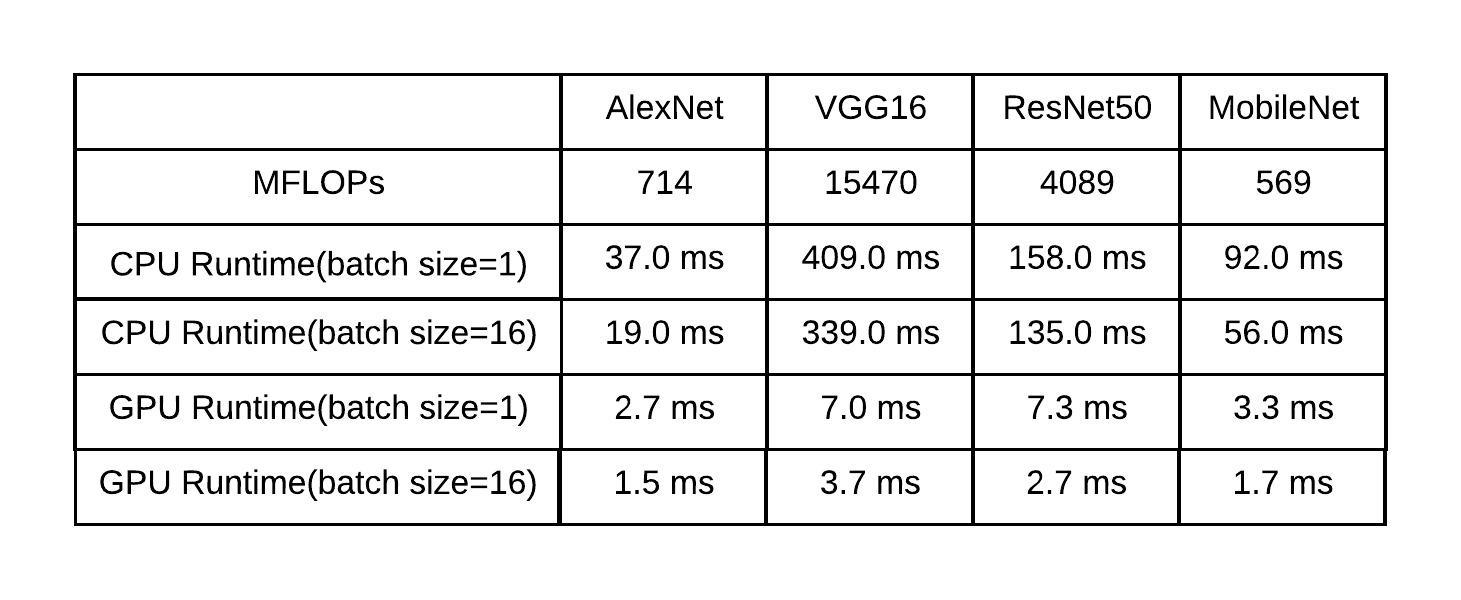
\includegraphics[width=\columnwidth]{./images/compute_cost}
  \caption{Compute cost of widely used Deep CNNs. (CPU: Intel(R) Core(TM) i7-6700 CPU \@ 3.40GHz machine with 32 GB Ram, GPU: Nvidia Titan Xp, Deep Learning Library: PyTorch 0.3.1)}
  \label{fig:compute_cost}
\end{figure}